\documentclass{beamer}

\usepackage{amsmath}
\usetheme{Szeged}
\usecolortheme{beaver}

\title[Fluid rendering with curvature flow] % (optional, only for long titles)
{Screen space fluid rendering with curvature flow}
\author[Musters, Terpstra] % (optional, for multiple authors)
{Bram Musters \and Maarten Terpstra}
\date{\today}
\subject{Computing Science}

\begin{document}
	\frame{\titlepage}
	\begin{frame}[t]\frametitle{Screen space fluid rendering}
		Screen space fluid rendering is performed using Smoothed Particle Hydrodynamics (SPH) 
	\end{frame}
	\begin{frame}[t]\frametitle{Curvature flow}
		Curvature flow is BLA
	\end{frame}
	\begin{frame}[t]\frametitle{Who, where and when?}
	    \begin{itemize}
	    	\item Wladimir J. van der Laan et al.
	    	\item NVIDIA 
	    	\item Rijksuniversiteit Groningen
	    	\item 2009
	    \end{itemize}
	\end{frame}
	\begin{frame}[t]\frametitle{Why?}
		\begin{itemize}
			\item Games
			\item No
		\end{itemize}
	\end{frame}
	\begin{frame}[t]\frametitle{Related work}
			
	\end{frame}
	\begin{frame}[t]\frametitle{Overview of method}
	    \begin{enumerate}
	    	\item Surface depth is written to render target
	    	\item Surface depth is smoothed
	    	\item Thickness is written to second render target
	    	\item Dynamic noise texture is generated on the surface of the fluid
	    	\item Smoothed surface depth, noise texture and an image of the scene behind the fluid is combined into the final rendering fluid 
	    \end{enumerate}	
	\end{frame}
	\begin{frame}[t]\frametitle{Surface depth}
		\begin{itemize}
			\item Particles rendered as spheres
			\item Native depth test
			\item No explicit splatting
			% Refer to practical where normals and colors are splatted.
			% The reason for this is that the depth values will be manipulated by the smoothing step.
			% This means that the normals will also change in the smoothing step.
		\end{itemize}	
	\end{frame}
	\begin{frame}[t]\frametitle{Surface depth smoothing}
	    \begin{itemize}
	    	\item Remove jelly-like appearance
	    	% To obtain a smooth flat surface
	    	\item Gaussian blur is unsuitable
	    	% When using straightforward gaussian kernels
	    	% Blurring will also occur on silhouette edges
	    	% Plateaus when using large kernels
	    	% Bilateral filters preserve edges, but are inefficient
	    	\item Curvature flow
	    \end{itemize}
	\end{frame}
	\begin{frame}[t]\frametitle{Curvature flow}
		\begin{itemize}
			\item Minimize curvature
			% This corresponds with nature, where surface tension create water drops and puddles.
			\item Transform the surface along its normal direction 
			\item \textbf{Screen-space}: transform the surface along the $z$ direction 
			% Normally, the surface is transformed along the normal direction of the surface,
			% but since we are working in the depth buffer, this is the z direction
			\item Amount of transformation depends on the magnitude of the mean curvature
		\end{itemize}
		\begin{equation}
			\frac{\partial z}{\partial t} = H
		\end{equation}
		% t is the smoothing time step, H is mean curvature
		\begin{equation}
			H = \frac{\nabla \cdot \hat{n}}{2}
		\end{equation}
		% Mean curvature is defined as the divergence of the unit normal of a surface
	\end{frame}
	\begin{frame}[t]\frametitle{Thickness}
	    \begin{itemize}
	    	\item Objects become less visible if water is in front of it
	    	\item Attenuate colour of object based on "thickness"
	    	\begin{equation}
	    		T(x, y) = \sum_{i = 0}^{n} d(\frac{x - x_i}{\sigma_i}, \frac{y - y_i}{\sigma_i})
	    	\end{equation}
	    	\item Additive blending based on this measure
	    \end{itemize}
	\end{frame}
	\begin{frame}[t]\frametitle{Noise}
	    \begin{itemize}
	    	\item Smooth surfaces are unrealistic
	    	\item Add noise to surface to add detail
	    	\item Assign Perlin noise to each particle
	    	\item Make them contribute less as they submerge
	    \end{itemize}
	\end{frame}
	\begin{frame}[t]\frametitle{Results}
	    \begin{itemize}
	    	\item 64000 particles
	    	\item 2-3 times slower than Gaussian smoothing
	    	\item Much better results
	    \end{itemize}
	\end{frame}
	\begin{frame}[t]\frametitle{Results}
	    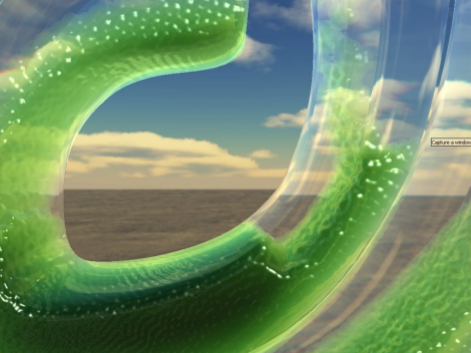
\includegraphics[scale=.5]{gaussian.png}
	\end{frame}
	\begin{frame}[t]\frametitle{Results}
	    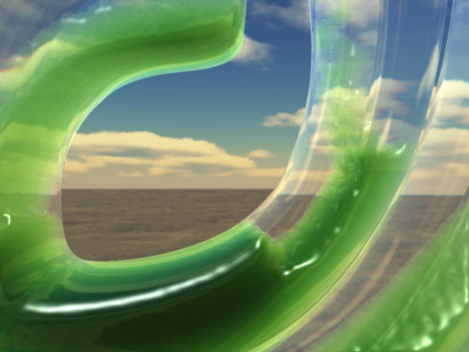
\includegraphics[scale=.5]{curveFlow.png}
	\end{frame}
\end{document}